\documentclass[a4paper,12pt]{report}
\usepackage{a4wide}

%\documentclass[a5paper,10pt]{book}
%\usepackage[top=23mm, bottom=18mm, left=15mm, right=25mm]{geometry}
%\geometry{papersize={170mm,220mm}}


\usepackage[utf8x]{inputenc}
\usepackage[danish]{babel}

\usepackage{xr-hyper} %Externe hyper-ref
\usepackage[colorlinks=true, hyperindex=true, linkcolor=minmblaa, citecolor=minmblaa, urlcolor=minmblaa]{hyperref}
\hypersetup{colorlinks=true,filecolor=minmblaa,bookmarksnumbered=true} %Til hyperreferencer. Referencer med farver
\usepackage{needspace} % giver mulighed for at kræve at der skal være et antal tomme linier på siden før ellers indsættes et sideskift.
\usepackage{framed} %Bokse
\usepackage{wrapfig}

\usepackage{amsmath,amsfonts,amssymb,amsthm,mathtools} %Matematikpakker

\setlength{\parindent}{0mm} %Ingen Indhak i første linje i afsnit

\usepackage{color} %Farvepakke

\usepackage{array}
\usepackage{colortbl}
\usepackage{multirow} %Til at flette rækker i tabeller.

\usepackage{verbatim,mhchem}



	% DOWNLOAD FRA: http://sarovar.org/frs/?group_id=52&release_id=97
	% Læg i directory for hoved TEX fil
%\usepackage[draft]{pdfdraftcopy}
%\draftstring{Licens: Kasper Langt Mellemnavn Skårhøj}
%\draftfontsize{30}
	%\draftfontfamily{hlh}
	%\draftangle{45}
	%\definecolor{mycolor}{rgb}{.825,.855,1}
	%\draftcolor{mycolor}
	%\draftfontattrib



% = Sidehoved =
\usepackage{fancyhdr}
\pagestyle{fancy}
\renewcommand{\sectionmark}[1]{\markright{\protect\titlegraphic{dturoed}\textcolor{dtugraa}{\thesection~\MakeUppercase{#1}}}} % \thesection.\
\fancyhead{}
\fancyfoot{}
\fancyhead[R]{\titlefont\thepage}
\fancyhead[C]{}
\fancyhead[L]{\titlefont \small eNote \MakeUppercase{~\thechapter}~\hspace*{1ex}\rightmark}
\renewcommand\headrulewidth{0pt}
\fancypagestyle{plain}{\fancyfoot[C]{}}% {\titlefont\footnotesize\thepage}}
\setlength{\headheight}{15pt}


% = Længder
%\newlength{\envtblsep}\setlength{\envtblsep}{1\FrameSep}
\newlength{\obsl}\setlength{\obsl}{\textwidth-1.2cm-13.2pt}

% Includes:

% =     Fonts (select one)    =
\usepackage{mathpazo}\linespread{1.05} % Palatino needs more leading (space between lines)
\usepackage{bm} % bold math, must be loaded after the fontpackages

% % Til overskrifter
\DeclareTextFontCommand{\th}{\fontencoding{T1}\fontfamily{phv}\fontseries{b}\selectfont}
\newcommand\titlefont{\fontencoding{T1}\fontfamily{phv}\selectfont}


% =     PGF grafik      =
\usepackage{tikz}
\newcommand\titlegraphic[1]{%
\tikz[baseline] %
\draw[thick,color=#1]
(0pt  ,-0.25em) -- (0pt  ,0.85em)
(2.5pt,-0.25em) -- (2.5pt,0.85em)
(5pt  ,-0.25em) -- (5pt  ,0.85em)
(7.5pt,-0.25em) -- (7.5pt,0.85em);\hspace*{0.8ex} %
}

\newcommand\titlegraphicwide[1]{%
\tikz[baseline] %
\draw[line width=0.8mm,color=#1]
(0pt  ,-0.25em) -- (0pt  ,0.85em)
(4.5pt,-0.25em) -- (4.5pt,0.85em)
(9pt  ,-0.25em) -- (9pt  ,0.85em)
(13.5pt,-0.25em) -- (13.5pt,0.85em);\hspace*{0.8ex} %
}


% =      Title Layout      =
\usepackage{titlesec}
\makeatletter
\titleformat{\chapter}
	[display] % Shape
	{\titlefont\Huge\flushleft} % Title and label format
	{\titlefont\LARGE\bfseries \titlegraphicwide{dturoed}\textcolor{dtugraa}{\@chapapp~\thechapter}} % label
	{0.9em} % label/title separation
	{} % before code
	[] % after code
\makeatother
\titleformat{\section}
	[hang] % Shape
	{\titlefont\Large\flushleft} % Title and label format
	{\thesection} % label
	{0.9em} % label/title separation
	{} % before code
	[] % after code
\titleformat{\subsection}
	[hang] % Shape
	{\titlefont\large} % Title and label format
	{\thesubsection} % label
	{0.9em} % label/title separation
	{} % before code
	[] % after code
\titlespacing{\subsection}{0pt}{*6}{*1.5}
\titleformat{\subsubsection}
	[hang] % Shape
	{\titlefont} % Title and label format
	{\thesubsubsection} % label
	{0.9em} % label/title separation
	{} % before code
	[] % after code



% = Farver
\definecolor{dturoed}{rgb}{0.6, 0.0, 0.0}
\definecolor{dtugraa}{rgb}{0.5, 0.5, 0.5}	% Lidt mørkere. Korrekt = 0.4
\definecolor{mingroenstreg}{rgb}{0.4,0.8,0}	% Sekundærfarve 14 : 102/204/0	(Forårsgrøn) -> Eksempler
\definecolor{mingroen}{rgb}{0.32,0.64,0}		% Sekundærfarve 14, 80% mørkere (tekst)
\definecolor{minorangestreg}{rgb}{1,0.6,0}		% Sekundærfarve 1 : 255/153/0	(Orange) -> Opgaver
\definecolor{minorange}{rgb}{0.8,0.48,0}		% Sekundærfarve 1 , 80% mørkere (tekst)

\definecolor{minblaa}{rgb}{0.2,0.4,0.8}	% Sekundærfarve 13 , 51/102/204 	( Blå -> Definitioner etc)
\definecolor{minmblaa}{rgb}{0.16,0.32,0.64}	% Sekundærfarve 13 , 80% mørkere (tekst)
\definecolor{thmbackground}{rgb}{0.97,.97, 0.99}	% Farve 13 - lys baggrund

\definecolor{mingraastreg}{rgb}{.5,.5,.5}
\definecolor{hvadbackground}{rgb}{0.97,.97, 0.97}
\definecolor{sumgul}{rgb}{1,1,.8}

\definecolor{hjmopgfarve}{rgb}{.96,1,.96}


% = Counter
\newcounter{evncount}[chapter]
\setcounter{evncount}{0}
\renewcommand{\theevncount}{\thechapter.\arabic{evncount}}
\renewcommand{\theequation}{\thechapter-\arabic{equation}}


% = Eksempler = example =
\newenvironment{example}[1][]{
	\refstepcounter{evncount}
	\setlength{\obsl}{\textwidth-1.2cm-13.2pt-9pt} % fix width of the info envirnment%
	\def\FrameCommand{ 
		\textcolor{mingroenstreg}{\vrule width 4pt} 
		\hspace{5pt} 
	}%
	\MakeFramed{\advance\hsize-\width \FrameRestore}%
	\needspace{3\baselineskip}
	\titlegraphic{mingroen}
	\textcolor{mingroen}{
		\th{Eksempel \theevncount \hspace*{5mm} #1}
	} 
	\vspace*{3mm}%
	\begin{small}
	\par
}
{
	\end{small}
	\endMakeFramed
}


% = Opgaver = exercise =
\newenvironment{exercise}[1][]{
	\refstepcounter{evncount}
	\setlength{\obsl}{\textwidth-1.2cm-13.2pt-9pt}% fix width of the info envirnment%
	\def\FrameCommand{
		\textcolor{minorangestreg}{\vrule width 4pt}
		\hspace{5pt}
	}%
	\MakeFramed{\advance\hsize-\width \FrameRestore}%
	\needspace{3\baselineskip}
	\titlegraphic{minorange}
	\textcolor{minorange}{
		\th{Opgave \theevncount \hspace*{5mm} #1}
	} 
	\vspace*{3mm}%
	\begin{small}
	\par
}
{
	\end{small}
	\endMakeFramed
}


% = Bevis
\newenvironment{bevis}{
	\setlength{\obsl}{\textwidth-1.2cm-13.2pt-9pt} % fix width of the info envirnment%
	\def\FrameCommand{
		\textcolor{mingraastreg}{\vrule width 4pt} 
		\hspace{5pt}
	}%
	\MakeFramed{\advance\hsize-\width \FrameRestore}%
	\needspace{3\baselineskip}
	\titlegraphic{black}
	\textcolor{black}{
		\th{Bevis}
	}
	\vspace*{3mm}%
	\begin{small}
	\par
}
{
	\bevisslut 
	\end{small}
	\endMakeFramed
}


% = Definition =
\newenvironment{definition}[1][]{
	\vspace{4mm}
	\pagebreak[1]
	\setlength{\obsl}{\textwidth-1.2cm-2\FrameSep-13.2pt}%
	\def\FrameCommand{
		\fboxsep=\FrameSep\fcolorbox{minblaa}{thmbackground}
	}
	\begin{minipage}{\textwidth}
	\MakeFramed{\advance\hsize-\width\FrameRestore}
	\refstepcounter{evncount}
	\titlegraphic{minblaa}
	\textcolor{minmblaa}{
		\th{Definition \theevncount \hspace*{5mm} #1}
	}
	\vspace*{3mm}
	\par
}
{
	\endMakeFramed 
	\end{minipage}
	\vspace{4mm}
}


% = Theorem =
\newenvironment{theorem}[1][]{
	\vspace{4mm}
	\pagebreak[1]%
	\setlength{\obsl}{\textwidth-1.2cm-2\FrameSep-13.2pt}%
	\def\FrameCommand{
		\fboxsep=\FrameSep\fcolorbox{minblaa}{thmbackground}
	}%
	\begin{minipage}{\textwidth}
	\MakeFramed{\advance\hsize-\width\FrameRestore}%
	\refstepcounter{evncount}
	\titlegraphic{minblaa}
	\textcolor{minmblaa}{
		\th{Sætning \theevncount \hspace*{5mm} #1}
	}
	\vspace*{3mm}
	\par
}
{
	\endMakeFramed 
	\end{minipage}
	\vspace{4mm}
}


% = Lemma =
\newenvironment{lemma}[1][]{
	\vspace{4mm}
	\pagebreak[1]
	\setlength{\obsl}{\textwidth-1.2cm-2\FrameSep-13.2pt}%
	\def\FrameCommand{
		\fboxsep=\FrameSep \fcolorbox{minblaa}{thmbackground}
	}
	\begin{minipage}{\textwidth} 
	\MakeFramed{\advance\hsize-\width \FrameRestore}
	\refstepcounter{evncount}
	\titlegraphic{minblaa}
	\textcolor{minmblaa}{
		\th{Hjælpesætning \theevncount \hspace*{5mm} #1}
	}
	\vspace*{3mm}
	\par
}
{
	\endMakeFramed 
	\end{minipage}
	\vspace{4mm}
}


% = Corollary =
\newenvironment{corollary}[1][]{
	\vspace{4mm}
	\pagebreak[1]
	\setlength{\obsl}{\textwidth-1.2cm-2\FrameSep-13.2pt}%
	\def\FrameCommand{
		\fboxsep=\FrameSep \fcolorbox{minblaa}{thmbackground}
	}
	\begin{minipage}{\textwidth} 
	\MakeFramed{\advance\hsize-\width \FrameRestore}
	\refstepcounter{evncount}
	\titlegraphic{minblaa}
	\textcolor{minmblaa}{
		\th{Følgesætning \theevncount \hspace*{5mm} #1}
	}
	\vspace*{3mm}
	\par
}
{
	\endMakeFramed 
	\end{minipage}
	\vspace{4mm}
}


% = Metode = method
\newenvironment{method}[1][]{
	\vspace{4mm}
	\pagebreak[1]
	\setlength{\obsl}{\textwidth-1.2cm-2\FrameSep-13.2pt}%
	\def\FrameCommand{
		\fboxsep=\FrameSep \fcolorbox{black}{hvadbackground}
	}
	\begin{minipage}{\textwidth} 
	\MakeFramed{\advance\hsize-\width \FrameRestore}
	\refstepcounter{evncount}
	\titlegraphic{black}
	\textcolor{black}{
		\th{Metode \theevncount \hspace*{5mm} #1}
	}
	\vspace*{3mm}
	\par
}
{
	\endMakeFramed
	\end{minipage}
	\vspace{4mm}
}


% = Forklaring = explain =
\newenvironment{explain}[1][]{
	\vspace{4mm}
	\pagebreak[1]
	\setlength{\obsl}{\textwidth-1.2cm-2\FrameSep-13.2pt}%
	\def\FrameCommand{
		\fboxsep=\FrameSep \fcolorbox{black}{hvadbackground}
	}
	\MakeFramed{\advance\hsize-\width \FrameRestore}
	\refstepcounter{evncount}
	\titlegraphic{black}
	\textcolor{black}{
		\th{Forklaring \theevncount \hspace*{5mm} #1}
	}
	\vspace*{3mm}
	\par
}
{
	\endMakeFramed
	\vspace{4mm}
}


% = Bemærkning = remark =
\newenvironment{remark}[1][]{
	\vspace{4mm}
	\pagebreak[1]
	\setlength{\obsl}{\textwidth-1.2cm-2\FrameSep-13.2pt}%
	\def\FrameCommand{
		\fboxsep=\FrameSep \fcolorbox{black}{hvadbackground}
	}
	\begin{minipage}{\textwidth} 
	\MakeFramed{\advance\hsize-\width \FrameRestore}
	\refstepcounter{evncount}
	\titlegraphic{black}
	\textcolor{black}{
		\th{Bemærkning \theevncount \hspace*{5mm} #1}
	}
	\vspace*{3mm}
	\par
}
{
	\endMakeFramed 
	\end{minipage}
	\vspace{4mm}
}







% = OBS! = obs =
\newenvironment{obs}{\vspace{4mm}\par%
\begin{tabular}{m{1.2cm}<{\hspace*{2mm}}@{}|m{\obsl}@{}}\hspace*{-4pt}\raggedleft
\includegraphics[width=1.1cm]{../Strukturfiler/FIGS/Alert01} & \begin{minipage}{\obsl}}{\end{minipage}\\ \end{tabular}\vspace{4mm}\par}


% = INFO = info =
\newenvironment{info}{\vspace{4mm}\par%
\begin{tabular}{m{1.2cm}<{\hspace*{2mm}}@{}|m{\obsl}@{}}\hspace*{-4pt}\raggedleft
\includegraphics[width=1.1cm]{../Strukturfiler/FIGS/Info01} & \begin{minipage}{\obsl}}{\end{minipage}\\ \end{tabular}\vspace{4mm}\par}


% = THINK= think =
\newenvironment{think}{\vspace{4mm}\par%
\begin{tabular}{m{1.2cm}<{\hspace*{2mm}}@{}|m{\obsl}@{}}\hspace*{-4pt}\raggedleft
\includegraphics[width=0.7cm]{../Strukturfiler/FIGS/ChessPiece} & \begin{minipage}{\obsl}}{\end{minipage}\\ \end{tabular}\vspace{4mm}\par}


% = AHA= aha =
\newenvironment{aha}{\vspace{4mm}\par%
\begin{tabular}{m{1.2cm}<{\hspace*{2mm}}@{}|m{\obsl}@{}}\hspace*{-4pt}\raggedleft
\includegraphics[width=1.1cm]{../Strukturfiler/FIGS/Think} & \begin{minipage}{\obsl}}{\end{minipage}\\ \end{tabular}\vspace{4mm}\par}


% = BUILDUP= build =
\newenvironment{build}{\vspace{4mm}\par%
\begin{tabular}{m{1.2cm}<{\hspace*{2mm}}@{}|m{\obsl}@{}}\hspace*{-4pt}\raggedleft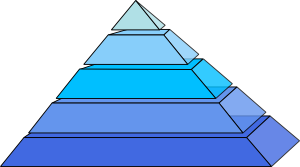
\includegraphics[width=1.1cm]{../Strukturfiler/FIGS/BluePyramid} & \begin{minipage}{\obsl}}{\end{minipage}\\ \end{tabular}\vspace{4mm}\newline}


% = Forudsætning = basis
\newenvironment{basis}{\begin{flushleft} \begin{itshape} }{\end{itshape} \end{flushleft}}


% = Opsummering =
\newenvironment{summary}{\clearpage\pagecolor{sumgul}\section{Opsummering}}{\newpage\pagecolor{white}}











% = Counter
\newcounter{opgavecount}[section]
\setcounter{opgavecount}{0}
\newcounter{spgcount}[opgavecount]
\setcounter{spgcount}{0}
\renewcommand{\thespgcount}{\alph{spgcount})}



% = EXERCISE = (DIVIDER)

\newcommand{\exercisebegin}[1][]{\bigskip\needspace{3\baselineskip}\refstepcounter{opgavecount}\titlegraphic{mingroen}\textcolor{mingroen}{\th{Opgave \theopgavecount \hspace*{1cm} #1}}\medskip\par}

% = QUIZEXERCISE = (DIVIDER)

\newcommand{\quizexercisebegin}[1][]{\bigskip\needspace{3\baselineskip}\refstepcounter{opgavecount}\titlegraphic{mingroen}\textcolor{mingroen}{\th{Quiz-Opgave \theopgavecount \hspace*{1cm} #1}}\medskip\par}

% = QUESTION =

\newenvironment{question}{\refstepcounter{spgcount}\begin{itemize}\item[\thespgcount]}{\end{itemize}\hspace*{\fill}}

% = VINK =

\newenvironment{vink}{\begin{tabular}{m{.9cm}<{\hspace*{2mm}}@{}|m{\obsl}@{}}\hspace*{-4pt}\raggedleft
\includegraphics[width=.9cm]{../Strukturfiler/FIGS/Think} & \begin{minipage}{\obsl}}{\end{minipage}\\ \end{tabular}\medskip\\}
	
% = FACIT =

\newenvironment{facit}{\begin{tabular}{m{.9cm}<{\hspace*{2mm}}@{}|m{\obsl}@{}}\hspace*{-4pt}\raggedleft
\includegraphics[width=.9cm]{../Strukturfiler/FIGS/Check} & \begin{minipage}{\obsl}}{\end{minipage}\\ \end{tabular}\medskip\\}








\newcommand{\afsnit}[1]{\bigskip\th{\titlegraphic{mingroen}\textcolor{mingroen}{#1}} \\ \rule[7pt]{.4\textwidth}{1pt} \vspace*{-2.5mm}\par}

% (DIVIDER):
\newcommand{\ugedagdatotitel}[4]{\pagebreak[4]\section{Semesteruge #1 -- #2 Dag \hspace*{1mm} (#3)} \vspace*{-4mm} \rule[5pt]{\textwidth}{1pt}\vspace*{-2.5mm} \begin{center}\large{\th{#4}}\end{center} \fancyhead[C]{\th{Semesteruge #1}}}

\newenvironment{skema}[1]{\definecolor{shadecolor}{rgb}{0.96,.98, 1.0} \setlength{\FrameSep}{6pt} \renewcommand{\FrameHeightAdjust}{10pt} \vspace*{-4pt}\begin{shaded} \begin{tabular}{#1}}{\end{tabular} \end{shaded} \vspace*{-7pt}}


% ========================

% MAKROER

%\newenvironment{matr}[1][]{\hspace*{-.8mm}\left[\hspace*{-1mm}\begin{array}{#1}}{\end{array}\hspace*{-1mm}\right]\hspace*{-.8mm}}
\newcommand{\bevisslut}{\begin{scriptsize} \begin{flushright} $ \blacksquare $ \end{flushright} \end{scriptsize}}

\newcommand{\tref}[2]{\hyperref[#1]{#2 \ref*{#1}}}
\newcommand{\thref}[2]{\hyperref[#1]{#2}}

\newcommand{\refA}[1]{\colorbox{yellow}{\ref{#1}}}
\newcommand{\hrefA}[2]{\colorbox{yellow}{\href{#1}{#2}}}
\newcommand{\trefA}[2]{\colorbox{yellow}{\hyperref[#1]{#2 \ref*{#1}}}}
\newcommand{\threfA}[2]{\colorbox{yellow}{\hyperref[#1]{#2}}}

\newenvironment{matr}[1]{\hspace*{-.8mm}\begin{bmatrix}\hspace*{-1mm}\begin{array}{#1}}{\end{array}\hspace*{-1mm}\end{bmatrix}\hspace*{-.8mm}}
\newcommand{\transp}{\hspace*{-.6mm}^{\top}}

\newcommand{\maengde}[2]{\left\lbrace \hspace*{-1mm} \begin{array}{c|c} #1 & #2 \end{array} \hspace*{-1mm} \right\rbrace}

\newenvironment{eqnalign}[1]{\setlength{\arraycolsep}{1.3pt}\begin{equation}\begin{array}{#1}}{\end{array}\end{equation}\par}
\newcommand{\eqnl}{\setlength{\arraycolsep}{1.3pt}}

\newcommand{\matind}[3]{{_\mathrm{#1}\mathbf{#2}_\mathrm{#3}}}
\newcommand{\vekind}[2]{{_\mathrm{#1}\mathbf{#2}}}
\newcommand{\jac}[2]{{\mathrm{Jacobi}_\mathbf{#1} (#2)}}
\newcommand{\diver}[2]{{\mathrm{div}\mathbf{#1} (#2)}}
\newcommand{\rot}[1]{{\mathbf{rot}\mathbf{(#1)}}}

\newcommand{\am}{\mathrm{am}}
\newcommand{\gm}{\mathrm{gm}}
\newcommand{\E}{\mathrm{E}}
\newcommand{\Span}{\mathrm{span}}
\newcommand{\mU}{\mathbf{U}}

\newcommand{\ms}{\medskip\\}
\newcommand{\bs}{\bigskip\\}

\newcommand{\mA}{\mathbf{A}}
\newcommand{\mB}{\mathbf{B}}
\newcommand{\mC}{\mathbf{C}}
\newcommand{\mD}{\mathbf{D}}
\newcommand{\mE}{\mathbf{E}}
\newcommand{\mF}{\mathbf{F}}
\newcommand{\mK}{\mathbf{K}}
\newcommand{\mI}{\mathbf{I}}
\newcommand{\mM}{\mathbf{M}}
\newcommand{\mN}{\mathbf{N}}
\newcommand{\mQ}{\mathbf{Q}}
\newcommand{\mT}{\mathbf{T}}
\newcommand{\mV}{\mathbf{V}}
\newcommand{\mW}{\mathbf{W}}
\newcommand{\mX}{\mathbf{X}}
\newcommand{\ma}{\mathbf{a}}
\newcommand{\mb}{\mathbf{b}}
\newcommand{\mc}{\mathbf{c}}
\newcommand{\md}{\mathbf{d}}
\newcommand{\me}{\mathbf{e}}
\newcommand{\mn}{\mathbf{n}}
\newcommand{\mr}{\mathbf{r}}
\newcommand{\mv}{\mathbf{v}}
\newcommand{\mw}{\mathbf{w}}
\newcommand{\mx}{\mathbf{x}}
\newcommand{\mxb}{\mathbf{x_{bet}}}
\newcommand{\my}{\mathbf{y}}
\newcommand{\mz}{\mathbf{z}}
\newcommand{\reel}{\mathbb{R}}
\newcommand{\mL}{\bm{\Lambda}} %Lambda-matrix
\newcommand{\mnul}{\bm{0}}
\newcommand{\trap}[1]{\mathrm{trap}(#1)}
\newcommand{\Det}{\operatorname{Det}}
\newcommand{\adj}{\operatorname{adj}}
\newcommand{\Ar}{\operatorname{Areal}}
\newcommand{\Vol}{\operatorname{Vol}}
\newcommand{\Rum}{\operatorname{Rum}}
\newcommand{\diag}{\operatorname{\bf{diag}}}
\newcommand{\bidiag}{\operatorname{\bf{bidiag}}}
\newcommand{\spanVec}[1]{\mathrm{span}\{#1\}}
\newcommand{\Div}{\operatorname{Div}}
\newcommand{\Rot}{\operatorname{\mathbf{Rot}}}

\newcommand{\Jac}{\operatorname{Jacobi}}
\newcommand{\Tan}{\operatorname{Tan}}
\newcommand{\Ort}{\operatorname{Ort}}
\newcommand{\Flux}{\operatorname{Flux}}
\newcommand{\Cmass}{\operatorname{Cm}}
\newcommand{\Imom}{\operatorname{Im}}
\newcommand{\Pmom}{\operatorname{Pm}}
\newcommand{\IS}{\operatorname{I}}
\newcommand{\IIS}{\operatorname{II}}
\newcommand{\IIIS}{\operatorname{III}}
\newcommand{\Le}{\operatorname{L}}
\newcommand{\app}{\operatorname{app}}
\newcommand{\M}{\operatorname{M}}
\newcommand{\re}{\mathrm{Re}}
\newcommand{\im}{\mathrm{Im}}

\newcommand{\compl}{\mathbb{C}} %de komplekse tal
\newcommand{\e}{\mathrm{e}} %eksponentialfunktionen. lodret 'e', og altså ikke kursiv ligesom andre bogstaver.





% Medialink: SCREEN: (QRcode) + thumbnail image + link på kodenummer (til qr.dtu.dk)
\newcommand{\onlinemedia}[3]{
	\begin{wrapfigure}{r}{3.2cm} 
		\vspace{-30pt} 
		\vspace{#1pt} 
		\begin{flushright} 
			\includegraphics[width=3cm]{qr/#2.png} 
			\tiny 
			\href{http://qr.dtu.dk/#2}{#2: #3}
			\normalsize  
		\end{flushright} 
		\vspace{-10pt} 
	\end{wrapfigure}
}
\newcommand{\onlinemediathumb}[3]{
	\begin{wrapfigure}{r}{3.2cm} 
		\vspace{-30pt} 
		\vspace{#1pt} 
		\begin{flushright} 
			\includegraphics[width=3cm]{qr/#2.png} 
			\includegraphics[width=3cm]{qr/#2_thumb.png} 
			\tiny 
			\href{http://qr.dtu.dk/#2}{#2: #3}
			\normalsize  
		\end{flushright} 
		\vspace{-10pt} 
	\end{wrapfigure}
}



% Index:
\usepackage{makeidx}
\makeindex
\newcommand\ind[2]{\index{#1}\textbf{\textit{\textcolor{black}{#2}}}}

% ###SERVER_EXCLUDE_BEGIN###
\externaldocument[NUID17-]{../../enoten/TN01-Talrum/Talrum}
\externaldocument[NUID1-]{../../enoten/TN02-Ligningssystemer/TNdriver}
\externaldocument[NUID2-]{../../enoten/TN03-Matricer_og_Matrixalgebra/Matricer_og_matrixalgebra}
\externaldocument[NUID3-]{../../enoten/TN04-Kvadratiske_matricer/TNdriver}
\externaldocument[NUID11-]{../../enoten/TN05-Determinanter/Determinanter}
\externaldocument[NUID12-]{../../enoten/TN06-GeometriskeVektorer/GeometriskeVektorer}
\externaldocument[NUID18-]{../../enoten/TN07-Vektorrum/VektorRum}
\externaldocument[NUID21-]{../../enoten/TN08-LinAfbildninger/LinAfbildninger}
\externaldocument[NUID23-]{../../enoten/TN09-Egenvaerdier_og_egenvektorer/TNdriver}
\externaldocument[NUID24-]{../../enoten/TN10-Diagonalisering_med_egenvektorer/TNdriver}
\externaldocument[NUID10-]{../../enoten/TN11-1.ordens_differentialligninger/TNdriver}
\externaldocument[NUID13-]{../../enoten/TN12-1.ordens_differentialligningssystemer/TNdriver}
\externaldocument[NUID14-]{../../enoten/TN13-2.ordens_differentialligninger/TNdriver}
\externaldocument[NUID27-]{../../enoten/TN14-Elemenataere_funktioner/Elementaere_Funktioner}
\externaldocument[NUID28-]{../../enoten/TN15-Funktioner2Variable/Funktioner_To_Variable}
\externaldocument[NUID29-]{../../enoten/TN16-Gradienter_og_Tangentplaner/Gradienter_og_Tangentplaner}
\externaldocument[NUID32-]{../../enoten/TN17-Taylor_formler/Taylor_Formler}
\externaldocument[NUID33-]{../../enoten/TN18-Taylor_2Var/Taylor_2Var}
\externaldocument[NUID34-]{../../enoten/TN19-SymMat/SymmetriskeMatricer}
\externaldocument[NUID35-]{../../enoten/TN20-KegleSnit/Keglesnit}
\externaldocument[NUID36-]{../../enoten/TN21-Riemann_Integral/Riemann_01}
\externaldocument[NUID37-]{../../enoten/TN22-Plan_Int/Plan_Int_01}
\externaldocument[NUID39-]{../../enoten/TN23-Flade_Int/Flade_Rum_Int_01}
\externaldocument[NUID40-]{../../enoten/TN24-Vektorfelter/Vektorfelter_01}
\externaldocument[NUID41-]{../../enoten/TN25-Flux/Flux_02}
\externaldocument[NUID42-]{../../enoten/TN26-Gauss/Gauss_01}
\externaldocument[NUID128-]{../../enoten/TN27-Stokes/Stokes_01}
\externaldocument[NUID43-]{../../enoten/TN29-KomplekseTal/KomplekseTal}

\externaldocument[NUID6-]{../../E-math-opgaver/Opgaver/opgU123}
\externaldocument[NUID19-]{../../E-math-opgaver/Opgaver/opgU45}
\externaldocument[NUID20-]{../../E-math-opgaver/Opgaver/opgU678}
\externaldocument[NUID25-]{../../E-math-opgaver/Opgaver/opgU910SD}
\externaldocument[NUID31-]{../../E-math-opgaver/OpgaverF11-U123/opgF123}
% \externaldocument[NUID9-]{../../E-math-opgaver/Opgaver/Dagsordner E10}
% ###SERVER_EXCLUDE_END###


% Begin document and set alternative chapter title:
\begin{document}
\renewcommand{\chaptername}{eNote}

\setcounter{chapter}{11} %SÆT DETTE TAL TIL 1 MINDRE END DET AKTUELLE TRANSFERNOTE-NUMMER!!

%%%%%%%%%%%%%%%%%%%%%%%%%%%%%%%%%%%%%%%%%%%%
%%%%%%%%%%%%%%%%%%%%%%%%%%%%%%%%%%%%%%%%%%%%%
%%% HERFRA SKAL DU SKRIVE ELLER INDSÆTTE %%%%
%%% DEN FIL DU ØNSKER %%%%%%%%%%%%%%%%%%%%%%%
%%%%%%%%%%%%%%%%%%%%%%%%%%%%%%%%%%%%%%%%%%%%%
%%%%%%%%%%%%%%%%%%%%%%%%%%%%%%%%%%%%%%%%%%%%%

\chapter{Lineære 1. ordens differentialligningssystemer} \label{tn12}

\begin{basis}
Denne eNote beskriver 1. ordens differentialligningssystemer og viser, hvordan de kan løses. eNoten er i forlængelse af \tref{NUID10-tn11}{eNote}, der beskriver lineære differentialligninger generelt. Det er derfor en god idé at have læst den først. Desuden bruges egenværdier og -vektorer i løsningsproceduren, se \tref{NUID23-tn9}{eNote} og \tref{NUID24-tn10}{eNote}. 
\end{basis}

Vi vil her kigge på lineære koblede homogene differentialligninger af 1. orden med konstante koefficienter (se eventuelt forklaring \ref{hvad.diffsys21}). En sådan samling af \ind{koblede differentialligninger}{koblede differentialligninger} kaldes et \ind{differentialligningssystem}{differentialligningssystem}. Et differentialligningssystem af 1. orden med $ n $ ligninger ser principielt således ud:
\begin{equation}
\begin{matrix}
 x_1'(t) & = & a_{11}x_1(t) & + & a_{12}x_2(t) & + & \ldots & + & a_{1n}x_n(t) \\
 x_2'(t) & = & a_{21}x_1(t) & + & a_{22}x_2(t) & + & \ldots & + & a_{2n}x_n(t) \\
 \vdots  &   & \vdots       &   & \vdots       &   &        &   & \vdots       \\
 x_n'(t) & = & a_{n1}x_1(t) & + & a_{n2}x_2(t) & + & \ldots & + & a_{nn}x_n(t)
\end{matrix}
\end{equation}
I systemets venstreside er differentialkvotienterne af de $ n $ ukendte funktioner $ x_1(t) $, $x_2(t)$, $\ldots$, $x_n(t)$ linet op. Mens hver højreside er en linearkombination af de $n$ ukendte funktioner. Koefficienterne ($ a $'erne) er reelle konstanter. I matrix-format kan systemet skrives således:
\begin{equation}
\begin{matr}{c} x_1'(t) \\ x_2'(t) \\ \vdots \\ x_n'(t) \end{matr} = 
\begin{matr}{cccc} a_{11} & a_{12} & \ldots & a_{1n} \\
a_{21} & a_{22} & \ldots & a_{2n} \\
\vdots & \vdots & \ddots & \vdots \\
a_{n1} & a_{n2} & \ldots & a_{nn} \\ \end{matr} 
\begin{matr}{c} x_1(t) \\ x_2(t) \\ \vdots \\ x_n(t) \end{matr}
\end{equation}
Endnu mere kompakt skrives det
\begin{equation} 
\mx'(t) = \mA \mx(t)
\end{equation}
$ \mA $ kaldes \ind{systemmatrix}{systemmatricen}. Det er nu målet at løse et sådant differentialligningssystem, altså bestemme $ \mx(t) = (x_1(t), x_2(t), \ldots , x_n(t)) $. \bs
%Man kan også skrive systemet sådan:
%\begin{equation}
%f(\mx(t)) = \mx'(t) - \mA \mx(t) = 0
%\end{equation}
%På denne måde er det nemmere at se, at differentialligningssystemet er homogent -- der står nemlig ikke noget på højresiden og venstresiden indeholder kun led med den ukendte $ \mx(t) $.
%jævnføre REFERENCE (TN10 sætning 10.2 måske).
%Det overlades læseren at vise at differentialligningssystemet er lineært.

\begin{explain}[Hvad er et differentialligningssystem?] \label{hvad.diffsys21}
Differentialligningssystemer er samlinger af differentialligninger. Grunden til, at man ikke betragter differentialligningerne enkeltvis, er, at de ikke kan løses hver for sig, fordi de samme ukendte funktioner optræder i flere ligninger. Altså er ligningerne \textit{koblede}. En enkelt differentialligning fra et system kan for eksempel se således ud:
\begin{equation}
x_1'(t) = 4x_1(t) - x_2(t)
\end{equation}
Det er ikke muligt at bestemme hverken $ x_1(t) $ eller $ x_2(t) $, da der er to ukendte funktioner, men kun én differentialligning. \bs
For at kunne løse et sådant system fuldt ud, skal man have lige så mange ligninger, som man har ukendte funktioner (med deres tilhørende afledede). Den anden ligning i systemet kunne derfor være:
\begin{equation}
x_2'(t) = -6x_1(t) + 2x_2(t)
\end{equation}
Vi har nu lige så mange ligninger (to), som vi har ukendte funktioner (to), og det er nu muligt at bestemme både $ x_1(t) $ og $ x_2(t) $.\bs
For overskuelighedens skyld skriver man differentialligningssystemer på matrixform. Systemet ovenfor ser således ud:
\begin{equation}
\begin{matr}{c} x_1'(t) \\ x_2'(t) \end{matr} = \begin{matr}{rr} 4 & -1 \\ -6 & 2 \end{matr} \begin{matr}{c} x_1(t) \\ x_2(t) \end{matr} \quad \Leftrightarrow \quad \mx'(t) = \begin{matr}{rr} 4 & -1 \\ -6 & 2 \end{matr} \mx(t) = \mA \mx(t)
\end{equation}
Ser man bort fra, at det er vektorer og matricer, der opereres med, ligner ligningssystemet noget, vi har set før: $ x'(t) = A \cdot x(t) $, som man allerede kunne løse i gymnasiet. Løsningen til denne differentialligning er triviel: $ x(t) = c \e^{At} $, hvor $ c $ er en arbitrær konstant. Nedenfor finder vi ud af, at løsningen til det tilsvarende system af differentialligninger er sammenlignelig med $ x(t) = c \e^{At}\, $.\end{explain}

Vi løser nu differentialligningssystemet i følgende sætning. Sætningen indeholder forudsætninger, der ikke altid er opfyldte. De særtilfælde hvor sætningen ikke gælder, undersøges senere. Beviset for sætningen indeholder en meget kendt og brugt metode, kaldet \ind{diagonaliseringsmetoden}{diagonaliseringsmetoden}.

\begin{theorem} \label{saet.diffsys.egnv1}
Et lineært differentialligningssystem bestående af $ n $ ligninger med i alt $ n $ ukendte funktioner er givet ved
\begin{equation} \label{lig.saet.difflig1}
\mx'(t) = \mA \mx(t), \quad t \in \reel \,. 
\end{equation} 
Hvis $ \mA $ har $ n $ lineært uafhængige egenvektorer $ \mv _1, \mv _2, \ldots, \mv _n $ tilhørende (ikke nødvendigvis forskellige) egenværdier, $ \lambda_1, \lambda_2, \ldots, \lambda_n \,,$ er systemets fuldstændige løsningsmængde bestemt ved 
\begin{equation} \label{fuldKomplSol}
\mx(t) = c_1 \e^{\lambda_1 t} \mv_1 + c_2 \e^{\lambda_2 t} \mv_2 + \ldots + c_n \e^{\lambda_n t} \mv_n, \quad t \in \reel\,,
\end{equation}
hvor $ c_1, c_2, \ldots, c_n $ er vilkårlige komplekse konstanter:

\end{theorem}

\begin{obs}
Læg mærke til, at det ikke altid er muligt, at finde $ n $ lineært uafhængige egenvektorer. Derfor kan man ikke altid bruge sætning \ref{saet.diffsys.egnv1} til løsning af differentialligningssystemer af 1. orden. %Læg til gengæld mærke til at alle egenværdierne ikke behøver at være forskellige, det er kun egenvektorerne der skal være lineært uafhængige.
\bs
I sætningen er angivet den fuldstændige komplekse løsningsængde for differentialligningssystemet. Den fuldstændige reelle løsningsængde kan derefter findes som den reelle delmængde af den komplekse løsningsmængde. 
\end{obs}

\begin{bevis} \label{bev.diffsys.egnv1}
Vi gætter på, at en løsning til differentialligningssystemet $ \mx'(t) = \mA \mx(t) $ er en vektor $ \mv $ ganget på $ \e^{\lambda t} $, hvor $ \lambda $ er en konstant, så $ \mx(t) = \e^{\lambda t} \mv $. Vi har da den differentierede
\begin{equation} 
\mx'(t) = \lambda \e^{\lambda t} \mv \,.
\end{equation}
Sættes dette udtryk for $ \mx'(t) $ ind i ligning \eqref{lig.saet.difflig1} sammen med udtrykket for $ \mx(t) $ fås:
\begin{equation} 
\lambda \e^{\lambda t} \mv = \mA \e^{\lambda t} \mv \Leftrightarrow  \mA \mv - \lambda \mv = 0 \Leftrightarrow (\mA - \lambda \mE) \mv = 0 
\end{equation}
$ \e^{\lambda t} $ er forskellig for nul for ethvert $ t \in \reel $, hvorfor det kan divideres ud. Denne ligning er et egenværdiproblem. % REFERENCE. 
$ \lambda $ er en egenværdi til $ \mA $ og $ \mv $ er den tilhørende egenvektor. De kan begge bestemmes.
Det er nu lykkedes os at finde ud af, at $ \e^{\lambda t} \mv $ er én løsning til differentialligningssystemet, når $ \lambda $ er en egenværdi og $ \mv $ den tilhørende egenvektor til $ \mA $. \bs
Til at bestemme den fuldstændige løsningsmængde bruges den såkaldte \ind{diagonaliseringsmetoden}{diagonaliseringsmetode}: \bs
Vi antager, at $ \mA = \mA_{n \times n} $ har $ n $ lineært uafhængige (reelle eller komplekse) egenvektorer $ \mv_1, \mv_2, \ldots, \mv_n $ hørende til egenværdierne $ \lambda_1, \lambda_2, \ldots, \lambda_n $. Vi indfører nu den regulære matrix $ \mV $, som indeholder alle egenvektorerne:
\begin{equation} 
\mV = \begin{matr}{cccc} \mv_1 & \mv_2 & \cdots & \mv_n \end{matr}
\end{equation}
Endvidere indføres funktionen $ \my $, så $ \my(t) = ( y_1(t), y_2(t), \ldots, y_n(t) ) $, således at
\begin{equation} 
\mx(t) = \mV \my(t)
\end{equation} 
Vi har da, at $ \mx'(t) = \mV \my'(t) $. Indsættes disse udtryk for $ \mx(t) $ og $ \mx'(t) $ i ligning \eqref{lig.saet.difflig1}, fås
\begin{equation} 
\mV \my'(t) = \mA \mV \my(t) \Leftrightarrow \my'(t) = \mV^{-1} \mA \mV \my(t) = \mL \my(t), 
\end{equation}
hvor $ \mL = \mV^{-1} \mA \mV = \mathrm{diag}(\lambda_1, \lambda_2, \ldots \lambda_n) $ er en diagonalmatrix med egenværdierne tilhørende $ \mA $ %(REFERENCE OGSÅ DIAG!)
. \bs
Vi har nu ligningen $ \my'(t) = \mL \my(t) $, der kan skrives på følgende måde:
\begin{equation} 
\begin{aligned}
y_1'(t) &= \lambda_1 y_1(t) \\
y_2'(t) &= \lambda_2 y_2(t) \\
& \; \; \vdots \\
y_n'(t) &= \lambda_n y_n(t) \\
\end{aligned} 
\end{equation}
da $ \mL $ kun har elementer forskellig fra nul i diagonalen. Dette ligningssystem er ikke koblet: I hver ligning optræder kun én funktion og dens afledede. Derfor kan man løse dem enkeltvis, og den fuldstændige løsningsmængde til hver ligning er $ y(t) = c\e^{\lambda t} $ for alle $ c \in \compl $. Samlet giver det den fuldstændige løsningsmængde bestående af nedenstående funktioner for alle $ c_1,c_2,\ldots,c_n \in \compl $:
\begin{equation} 
\my(t) = \begin{matr}{c} y_1(t) \\ y_2(t) \\ \vdots \\ y_n(t) \end{matr} =
\begin{matr}{c} c_1\e^{\lambda_1 t} \\ c_2\e^{\lambda_2 t} \\ \vdots \\ c_n\e^{\lambda_n t} \end{matr}
\end{equation}
Da vi nu har løsningen $ \my(t) $ kan vi også finde løsningen $ \mx(t) = \mV \my(t) $:
\begin{equation} 
\begin{aligned}
\mx(t) &= \begin{matr}{cccc} \mv_1 & \mv_2 & \ldots & \mv_n \end{matr} \begin{matr}{c} c_1\e^{\lambda_1 t} \\ c_2\e^{\lambda_2 t} \\ \vdots \\ c_n\e^{\lambda_n t} \end{matr} \\
&= c_1 \e^{\lambda_1 t} \mv_1 + c_2 \e^{\lambda_2 t} \mv_2 + \ldots + c_n \e^{\lambda_n t} \mv_n \,.
\end{aligned} 
\end{equation}
Vi har nu fundet den fuldstændige komplekse løsningsmængde til ligningssystemet i ligning \eqref{lig.saet.difflig1} som består af funktionerne $ \mx(t) $ for alle $ c_1,c_2,\ldots,c_n \in \compl $.
%\begin{info}
%Man kommer nogle gange ud for at kunne bruge \textit{diagonaliseringsmetoden} i praksis i stedet for at gå direkte til løsningen i sætning \ref{saet.diffsys.egnv1}. For eksempel hvis der er problemer med antallet af egenvektorer. Man vil her kunne lave en tilsvarende matrix $ \mV $, der har en lidt anden form, og derefter kunne diagonalisere.
%\end{info}
\end{bevis}

\begin{example} \label{eks.diffsys1}
Der er givet differentialligningssystemet
\begin{eqnalign}{rcrcr}
x_1'(t) &=& x_1(t) &+& 2x_2(t) \\
x_2'(t) &=& 3x_1(t) & & 
\label{lig.eks.diffsys1} 
\end{eqnalign}
som på matrixform skrives som
\begin{equation} 
\mx'(t) = \begin{matr}{rr} 1 & 2 \\ 3 & 0 \end{matr} \mx(t) = \mA \mx(t).
\end{equation}
Det kan vises, at $ \mA $ har egenværdierne $ \lambda_1 = 3 $ og $ \lambda_2 = -2 $ med de tilhørende egenvektorer $ \mv_1 = ( 1, 1 ) $ og $ \mv_2 = (2, -3) $ (prøv selv!). Derfor er den fuldstændige reelle løsningsmængde 
%$ L_{hom} $
til differentialligningssystemet givet ved nedenstående funktioner for alle $ c_1,c_2 \in \reel $:
\begin{equation} 
\mx(t) = \begin{matr}{c} x_1(t) \\ x_2(t) \end{matr} = c_1\e^{3t} \begin{matr}{r} 1 \\ 1 \end{matr} + c_2\e^{-2t} \begin{matr}{r} 2 \\ -3 \end{matr} \, ,\quad t \in \reel
\end{equation}
Løsningen er fundet ved brug af sætning \ref{saet.diffsys.egnv1}. %Her har det kun interesse at de arbitrære konstanter er reelle, da vi ønsker reelle funktioner.
En anden måde at opskrive løsningsmængden på er ved at skille ligningssystemet ad, så
\begin{eqnalign}{rcrcr}
x_1(t)&=&c_1\e^{3t} &+& 2c_2\e^{-2t}\\
x_2(t)&=&c_1\e^{3t} &-& 3c_2\e^{-2t}
\end{eqnalign}
udgør løsningsmængden, hvor $ t \in \reel $, for alle $ c_1,c_2 \in \reel $. \bs
%Endvidere er en tredje måde at opskrive den fuldstændige løsningsmængde:
%\begin{equation}
%L_{hom} =  \maengde{c_1\e^{3t} \begin{matr}{r} 1 \\ 1 \end{matr} + c_2\e^{-2t} \begin{matr}{r} 2 \\ -3 \end{matr}}{t \in \reel, c_1,c_2 \in \reel}
%\end{equation}
\end{example}




\section{To koblede differentialligninger} \label{sek.diffsys.struktur1}

Givet et lineært homogent 1. ordens differentialligningssystem med konstante koefficienter med $ n $ ligninger og $ n $ ukendte funktioner
\begin{equation}
\mx'(t) = \mA \mx(t)\,. \quad t \in \reel
\end{equation}
Hvis systemmatricen $\mA$ har $n$ lineært uafhængige egenvektorer, kan systemets reelle løsningsmængde findes ved hjælp af sætning \ref{saet.diffsys.egnv1}. Hvis egenværdierne er reelle, kan den reelle løsningsmængde umiddelbart opskrives efter sætningens formel (\ref{fuldKomplSol}), hvor de de $n$ tilhørende lineært uafhængigge egenvektorer er reelle, og de arbitrære konstanter angives som reelle. Hvis systemmatricen har egenværdier som ikke er reelle, kan den reelle løsningsmænde finde2 ved at uddrage den reelle delmængde af den komplekse løsningsmængde. Også i dette tilfælde vil løsningsmængden kunne opskrives som en linearkombination af $n$ lineært uafhængige reelle løsninger til differentialligningssystem.\bs
Tilbage har vi særtilfældet, hvor systemmatricen ikke har $n$ lineært uafhængige egenvektorer. Også her vil den reelle løsningsmængde være en linearkombination af $n$ lineært uafhængige reelle løsninger til differentialligningssystemet. Her kan diagonaliseringsmetoden af gode grunde ikke benyttes, og man må bruge andre metoder.\bs
I dette afsnit gennemgår vi de nævnte tre tilfælde for  systemer der består af $ n = 2 $ koblede differentialligninger med $2$ ukendte funktioner.

\begin{method} \label{saet.diffsys.strukturloes1}
Den fuldstændige reelle løsningsmængde til differentialligningssystemet
\begin{equation}
\mx'(t) = \mA \mx(t), \quad t \in \reel,
\end{equation}
bestående af $ n = 2 $ ligninger med $2$ ukendte funktioner, kan opskrives som 
\begin{equation}
\mx(t) = c_1 \mathbf u_1(t) + c_2 \mathbf u_2(t)\,, \quad t \in \reel,
\end{equation}
hvor $\mathbf u_1 $ og $\mathbf u_2 $ er reelle lineært uafhængige partikulære løsninger og $ c_1,c_2 \in \reel $.\bs
Bestem først egenværdierne til $ \mA $. For rødderne i det karakteristiske polynomium $ \mA $ foreligger der tre muligheder:
\begin{itemize}
\item \textbf{To reelle enkeltrødder.} I så fald har begge egenværdier $ \lambda_1 $ og $ \lambda_2 $ algebraisk multiplicitet $1$ og geometrisk multiplicitet $1$, og vi kan sætte
\begin{equation}
\mathbf u_1(t) = \e^{\lambda_1 t} \mv_1 \quad \mathrm{og} \quad \mathbf u_2(t) = \e^{\lambda_2 t} \mv_2,
\end{equation}
hvor $ \mv_1 $ og $ \mv_2 $ er egentlige egenvektorer tilhørende $ \lambda_1 $ og $ \lambda_2 $ respektivt.
\item \textbf{To komplekse rødder.} De to egenværdier $ \lambda $ og $ \bar{\lambda} $ er da hinandens konjugerede komplekse tal. Vi bestemmer da $ \mathbf u_1 $ og $ \mathbf u_2 $ ved hjælp af metode \ref{saet.diffsys.kompleks1}.
\item \textbf{En dobbeltrod.} Her har egenværdien $ \lambda $ algebraisk multiplicitet $2$. Hvis den geometriske multiplicitet af $\lambda$ er $1$, bestemmes $ \mathbf u_1 $ og $ \mathbf u_2 $ ved hjælp af metode \ref{saet.diffsys.dobbeltrod1}.
\end{itemize}
\end{method}
 
Ved den første mulighed i metode \ref{saet.diffsys.strukturloes1} med to forskellige reelle egenværdier, kan man udmiddelbart benytte sætning \ref{saet.diffsys.egnv1}, idet de arbitrære konstanter vælges som reelle, se eksempel \ref{eks.diffsys1}. \bs

Nu følger metoden, der tager sig af tilfældet med to komplekse egenværdier.

\begin{method} \label{saet.diffsys.kompleks1}
To lineært uafhængige reelle løsninger til differentialligningssystemet
\begin{equation}
\mx'(t) = \mA \mx(t), \quad t \in \reel,
\end{equation}
hvor $ \mA $ har det komplekse egenværdipar $ \lambda = \alpha + \beta i $ og $ \bar{\lambda} = \alpha - \beta i $ med tilhørende egenvektorer $ \mv $ og $ \bar{\mv} $, er
\begin{equation}
\begin{aligned}
\mathbf u_1(t) &= \mathrm{Re}\left(\e^{\lambda t} \mv \right) = \e^{\alpha t} \left(\cos(\beta t) \mathrm{Re}(\mv) - \sin(\beta t) \mathrm{Im}(\mv) \right) \\
\mathbf u_2(t) &= \mathrm{Im}\left(\e^{\lambda t} \mv \right) = \e^{\alpha t} \left(\sin(\beta t) \mathrm{Re}(\mv) + \cos(\beta t) \mathrm{Im}(\mv) \right)
\end{aligned}
\end{equation}
\end{method}

Beviset medtages i næste version af denne eNote.

\begin{example} \label{eks.diffsys,kompleks1}
Givet differentialligningssystemet
\begin{equation}
\mx'(t) = \begin{matr}{rr} 1 & 1 \\ -1 & 1 \end{matr} \mx(t) = \mA \mx(t) \label{lig.eks.diffsys.kompleks1}
\end{equation}
Vi ønsker at bestemme den fuldstændige reelle løsningsmængde. \bs
Egenværdierne er bestemt til $ \lambda = 1 + i $ henholdsvis $ \bar{\lambda} = 1 - i $ med de tilhørende egenvektorer $ \mv = (-i,1) $ henholdsvis $ \bar{\mv} = (i,1) $. Det ses, at der er to komplekse egenværdier og dertil to komplekse egenvektorer. Med $ \lambda = 1 + i $ haves
\begin{equation}
\mv = \begin{matr}{r} -i \\ 1 \end{matr}  = \begin{matr}{r} 0 \\ 1 \end{matr} + i \begin{matr}{r} -1 \\ 0 \end{matr} = \re(\mv) + i \im(\mv)
\end{equation}
Bruges metode \ref{saet.diffsys.kompleks1} har vi da de to løsninger:
\begin{equation}
\mathbf u_1(t) = \e^{t} \left(\cos(t) \begin{matr}{r} 0 \\ 1 \end{matr} - \sin(t) \begin{matr}{r} -1 \\ 0 \end{matr} \right) = \e^{t} \begin{matr}{r} \sin(t) \\ \cos(t) \end{matr}
\end{equation}
\begin{equation}
\mathbf u_2(t) = \e^{t} \left(\sin(t) \begin{matr}{r} 0 \\ 1 \end{matr} + \cos(t) \begin{matr}{r} -1 \\ 0 \end{matr} \right) = \e^{t} \begin{matr}{r} -\cos(t) \\ \sin(t) \end{matr}
\end{equation}
Den fuldstændige reelle løsningsmængde til differentialligningssystemet \eqref{lig.eks.diffsys.kompleks1} er da givet ved følgende funktioner for alle $ c_1,c_2 \in \reel $:
\begin{equation}
\mx(t) = c_1\mathbf u_1(t) + c_2\mathbf u_2(t) = \e^{t} \left(c_1 \begin{matr}{r} \sin(t) \\ \cos(t) \end{matr} + c_2 \begin{matr}{r} -\cos(t) \\ \sin(t) \end{matr} \right), \quad t \in \reel
\end{equation}
fundet ved hjælp af metode \ref{saet.diffsys.strukturloes1}.
\end{example}
Endelig beskrives metoden der kan bruges, hvis systemmatricen har egenværdien $\lambda$ med am$(\lambda)=2$ og gm$(\lambda)=1$, dvs. hvor diagonalisering ikke mulig.

\begin{method} \label{saet.diffsys.dobbeltrod1}
Hvis systemmatricen $ \mA $ til differentialligningssystemet
\begin{equation}
\mx'(t) = \mA \mx(t), \quad t \in \reel,
\end{equation}
har en egenværdi $ \lambda $ med algebraisk multiplicitet 2, men det tilhørende egenvektorrum kun har geometrisk multiplicitet 1, findes to lineært uafhængige løsninger til differentialligningssystemet af formen:
\begin{equation}
\begin{aligned}
\mathbf u_1(t) &= \e^{\lambda t} \mv \\
\mathbf u_2(t) &= t \e^{\lambda t} \mv + \e^{\lambda t} \mb,
\end{aligned}
\end{equation}
hvor $ \mv $ er egenvektoren tilhørende egenværdien $ \lambda $, og $ \mb $ er løsning til nedenstående lineære ligningssystem:
\begin{equation}
(\mA - \lambda \mE)\mb = \mv
\end{equation}
\end{method}

\begin{bevis} \label{bev.diffsys.dobbeltrod1}
Det er åbenlyst, at den ene løsning til differentialligningssystemet er $ \mathbf u_1(t) = \e^{\lambda t} \mv $. Det svære er at finde endnu en løsning. \bs
Vi gætter på en løsning af formen
\begin{equation}
\mathbf u_2(t) = t \e^{\lambda t} \mv + \e^{\lambda t} \mb = \e^{\lambda t}(t \mv + \mb),
\end{equation}
hvor $ \mv $ er en egenvektor tilhørende $ \lambda $. Vi har da
\begin{equation}
\mathbf u_2\mathbf{'}(t) = (\e^{\lambda t} + \lambda t \e^{\lambda t})\mv + \lambda \e^{\lambda t} \mb = \e^{\lambda t}( (1 + \lambda t)\mv + \lambda \mb)
\end{equation}
Vi kontrollerer, om $ \mathbf u_2(t) $ er en løsning ved at indsætte det i $ \mx'(t) = \mA \mx(t) $:
\begin{equation}
\begin{aligned}
\mathbf u_2\mathbf{'}(t) &= \mA \mathbf u_2(t) \Leftrightarrow \\
(1 + \lambda t)\mv + \lambda \mb &= \mA (t \mv + \mb) \Leftrightarrow \\
t(\lambda \mv - \mA \mv ) + (\mv + \lambda \mb - \mA \mb) &= \mnul \Leftrightarrow \\
\lambda \mv - \mA \mv = \mnul \wedge \mv + \lambda \mb - \mA \mb &= \mnul
\end{aligned}
\end{equation}
Den første ligning kan nemt omformes til $ \mA \mv = \lambda \mv $, og den ses at være sand, da $ \mv $ er en egenvektor tilhørende $ \lambda $. Den anden ligning omformes:
\begin{equation}
\begin{aligned}
\mv + \lambda \mb - \mA \mb &= \mnul \Leftrightarrow \\
\mA \mb - \lambda \mb &= \mv \Leftrightarrow \\
(\mA - \lambda \mE)\mb &= \mv 
\end{aligned}
\end{equation}
Hvis $ \mb $ opfylder det foreskrevne ligningssystem, vil $ \mathbf u_2(t) $ også være en løsning til differentialligningssystemet. Vi har nu fundet to løsninger, og vi skal finde ud af, om de er lineært uafhængige. Dette gøres ved et normalt linearitetskriterium: Hvis ligningen $ k_1 \mathbf u_1 + k_2 \mathbf u_2 = \mnul $ kun har løsningen $ k_1=k_2=0 $ er $ \mathbf u_1 $ og $ \mathbf u_2 $ lineært uafhængige.
\begin{equation}
\begin{aligned}
k_1 \mathbf u_1 + k_2 \mathbf u_2 &= \mnul \Rightarrow \\
k_1 \e^{\lambda t} \mv + k_2 (t \e^{\lambda t} \mv + \mb \e^{\lambda t}) &= \mnul \Leftrightarrow \\
t(k_2 \mv) + (k_1 \mv + k_2 \mb) &= \mnul \Leftrightarrow \\
k_2 \mv = \mnul \wedge k_1 \mv + k_2 \mb &= \mnul
\end{aligned}
\end{equation}
Da $ \mv $ er en egenvektor, er den forskellig fra nulvektoren, og derfor er $ k_2 = 0 $ ifølge den første ligning. Den anden ligning er derved blevet reduceret til $ k_1 \mv = \mnul $, og med samme argument haves $ k_1 = 0 $. Derfor er de løsninger lineært uafhængige, og metoden er nu bevist.
\end{bevis}

\begin{example} \label{eks.diffsys.dobbeltrod1}
Givet differentialligningssystemet
\begin{equation}
\mx'(t) = \begin{matr}{rr} 16 & -1 \\ 4 & 12 \end{matr} \mx(t) = \mA \mx(t).
\end{equation}
Egenværdierne bestemmes for $ \mA $:
\begin{equation}
\begin{aligned}
\mathrm{det}(\mA - \lambda \mE) &= \begin{vmatrix} 16 - \lambda & -1 \\ 4 & 12 - \lambda \end{vmatrix} = (16 - \lambda)(12 - \lambda) + 4 \\
&= \lambda^2 - 28\lambda + 196 = (\lambda - 14)^2 = 0
\end{aligned}
\end{equation}
Der er altså kun én egenværdi, nemlig $ \lambda = 14 $, selvom det er et $ 2 \times 2 $-system. Egenvektorerne bestemmes:
\begin{equation}
\mA - 14 \mE = \begin{matr}{cc} 16-14 & -1 \\ 4 & 12-14 \end{matr} = \begin{matr}{rr} 2 & -1 \\ 4 & -2 \end{matr} \rightarrow \begin{matr}{rr} 1 & -\frac{1}{2} \\ 0 & 0 \end{matr}
\end{equation}
Man har da egenvektoren $ ( \frac{1}{2}, 1 ) $, eller $ \mv = ( 1, 2 ) $. Vi må altså konstatere, at egenværdien $ \lambda $ har algebraisk multiplicitet 2, men at det tilhørende vektorrum har geometrisk multiplicitet 1. For at bestemme to uafhængige løsninger til differentialligningsystemet kan metode \ref{saet.diffsys.dobbeltrod1} bruges. \bs
Først løses følgende ligningssystem:
\begin{equation}
(\mA - \lambda \mE)\mb = \mv \Rightarrow \begin{matr}{rr} 2 & -1 \\ 4 & -2 \end{matr} \mb = \begin{matr}{rr} 1 \\ 2 \end{matr}
\end{equation}
\begin{equation}
\begin{matr}{rrr} 2 & -1 & 1 \\ 4 & -2 & 2 \end{matr} \rightarrow \begin{matr}{rrr} 1 & -\frac{1}{2} & \frac{1}{2} \\ 0 & 0 & 0 \end{matr}
\end{equation}
Dette giver $ \mb = (1, 1) $, hvis den frie variabel sættes til $ 1 $. De to løsninger er da
\begin{equation}
\begin{aligned}
\mathbf u_1(t) &= \e^{14 t} \begin{matr}{r} 1 \\ 2 \end{matr} \\
\mathbf u_2(t) &= t \e^{14 t} \begin{matr}{r} 1 \\ 2 \end{matr} + \e^{14 t} \begin{matr}{r} 1 \\ 1 \end{matr}.
\end{aligned}
\end{equation}
Ved hjælp af metode \ref{saet.diffsys.strukturloes1} kan den fuldstændige løsningsmængde bestemmes til at være følgende funktioner for alle $ c_1,c_2 \in \reel $:
\begin{equation}
\mx(t) = c_1\mathbf u_1(t) + c_2\mathbf u_2(t) = c_1 \e^{14 t} \begin{matr}{r} 1 \\ 2 \end{matr} + c_2 \e^{14 t} \left(t \begin{matr}{r} 1 \\ 2 \end{matr} + \begin{matr}{r} 1 \\ 1 \end{matr} \right).
\end{equation}
\end{example}
\section{n-dimensionalt løsningsrum}
I det foregående afsnit har vi betragtet koblede systemer bestående af to lineære ligningssystemer med to ukendte funktioner. Løsningsrummet er to-dimensionalt, idet det kan opskrives som en linearkombination af to lineært uafhængige løsninger. Dette kan generaliseres til vilkårlige systemer med $ n \geq 2 $ koblede lineære differentialligninger med $n$ ukendte funtioner: Løsningsmængden er en linearkombination af netop $ n $ lineært uafhængige løsninger. Dette formuleres i generel form i følgende sætning. %\ind{differentialligningssystem!struktursætning}{struktursætning}.  

\begin{theorem} \label{saet.diffsys.struktur1}
Givet det lineære homogene 1. ordens differentialligningssystem med konstante reelle koefficienter
\begin{equation}
\mx'(t) = \mA \mx(t), \quad t \in \reel,
\end{equation}
bestående af $ n $ ligninger og med i alt $ n $ ukendte funktioner. Den fuldstændige reelle løsningsmængde til systemet er $n$-dimensionalt kan opskrives ved
\begin{equation}
\mx(t) = c_1 \mathbf u_1(t) + c_2 \mathbf u_2(t) + \cdots + c_n \mathbf u_n(t),
\end{equation}
hvor $ \mathbf u_1(t),\mathbf u_2(t),\ldots,\mathbf u_n(t) $ er lineært uafhængige reelle løsninger til differentialligningssystemet, og $ c_1,c_2,\ldots,c_n \in \reel $.
\end{theorem}

Herunder er et eksempel med et koblet system af tre differentiallinger, der eksemplificerer sætning \ref{saet.diffsys.struktur1}.

\begin{example}[Advanced] \label{eks.diffsys.dob.enk1}
Givet differentialligningssystemet
\begin{equation}
\mx'(t) = \begin{matr}{rrr} -9 & 10 & 0 \\ -3 & 1 & 5 \\ 1 & -4 & 6 \end{matr} \mx(t) = \mA \mx(t)
\end{equation}
Vi ønsker at bestemme den fuldstændige reelle løsningsmængde til differentialligningssystemet. Egenværdierne og egenvektorene kan bestemmes og er som følger:
\begin{eqnarray}
\lambda_1 = -4 &:& \mv_1 = (10,5,1) \nonumber \\
\lambda_2 = 1 &:& \mv_2 = (5,5,3)\nonumber
\end{eqnarray}
Desuden har $ \lambda_2 $ algebraisk multiplicitet 2, men det tilhørende egenvektorrum har geometrisk multiplicitet 1. Fordi $ n=3 $ skal vi bruge 3 lineært uafhængige løsninger til at danne den fuldstændige løsningsmængde, som set i sætning \ref{saet.diffsys.struktur1}. Egenværdierne betragtes hver for sig: \bs
1) Den første egenværdi, $ \lambda_1 = -4 $, har både geometrisk og algebraisk multiplicitet lig 1. Det giver netop én løsning
\begin{equation}
\mathbf u_1(t) = \e^{\lambda_1 t} \mv_1 = \e^{-4t} \begin{matr}{r} 10 \\ 5 \\ 1 \end{matr} 
\end{equation}
2) Den anden egenværdi, $ \lambda_2 = 1 $, har algebraisk multiplicitet 2, men geometrisk multiplicitet 1. Derfor kan vi bruge metode \ref{saet.diffsys.dobbeltrod1} til at finde to løsninger. Først bestemmes $ \mb $:
\begin{equation}
(\mA - \lambda_2 \mE)\mb = \mv_2 \Rightarrow \begin{matr}{rrr} -10 & 10 & 0 \\ -3 & 0 & 5 \\ 1 & -4 & 5 \end{matr} \mb = \begin{matr}{r} 5 \\ 5 \\ 3 \end{matr}
\end{equation}
En partikulær løsning til dette ligningssystem er $ \mb = (0,\frac{1}{2},1) $. Med denne viden har vi yderligere to lineært uafhængige løsninger til differentialligningssystemet:
\begin{equation}
\begin{aligned}
\mathbf u_2(t) &= \e^{\lambda_2 t} \mv_2 = \e^{t} \begin{matr}{r} 5 \\ 5 \\ 3 \end{matr} \\
\mathbf u_3(t) &= t \e^{\lambda_2 t} \mv_2 + \e^{\lambda_2 t} \mb = t \e^{t} \begin{matr}{r} 5 \\ 5 \\ 3 \end{matr} + \e^{t} \begin{matr}{r} 0 \\ \frac{1}{2} \\ 1 \end{matr}
\end{aligned}
\end{equation}
Det er op til læseren at vise, at de tre løsninger er lineært uafhængige. \bs
Ifølge metode \ref{saet.diffsys.struktur1} er den fuldstændige reelle løsningsmængde udgjort af følgende linearkombination for alle $ c_1,c_2,c_3 \in \reel $:
\begin{equation}
\mx(t) = c_1 \mx_1(t) + c_2 \mx_2(t) + c_3 \mx_3(t)
\end{equation} 
Dette giver altså
\begin{equation}
\mx(t) = c_1 \e^{-4t} \begin{matr}{r} 10 \\ 5 \\ 1 \end{matr} + c_2 \e^{t} \begin{matr}{r} 5 \\ 5 \\ 3 \end{matr} + c_3 \left( t \e^{t} \begin{matr}{r} 5 \\ 5 \\ 3 \end{matr} + \e^{t} \begin{matr}{r} 0 \\ \frac{1}{2} \\ 1 \end{matr} \right)
\end{equation}
hvor $ t \in \reel $ og alle $ c_1,c_2,c_3 \in \reel $.
\end{example}

\section{Eksistens og entydighed af løsninger} \label{subsek.diffsys.eksent1}

Ifølge struktursætningen \ref{saet.diffsys.struktur1} indeholder den fuldstændige løsningsmængde til et differentialligningssystem med $ n $ ligninger $ n $ arbitrære konstanter. Hvis man har $ n $ \ind{begyndelsesværdibetingelse}{begyndelsesværdibetingelser}, så kan konstanterne bestemmes, og vi får da en entydig løsning. Dette formuleres i følgende \ind{differentialligningssystem!eksistens og entydighed}{eksistens- og entydighedssætning}.

\begin{theorem} \label{saet.diffsys.eksent1}
Et 1. ordens differentialligningssystem bestående af $ n $ ligninger og $ n $ ukendte funktioner med konstante koefficienter er givet ved
\begin{equation}
\mx'(t) = \mA \mx(t), \quad t \in I \,.
\end{equation}
For ethvert $t_0 \in I$ og ethvert talsæt $\mathbf y_0=(y_1,y_2,\ldots,y_n)$ findes der netop én løsning $\mx(t)=(x_1(t),x_2(t)\ldots,x_n(t)\,)$ der opfylder begyndelsesværdibetingelsen
\begin{equation}
\mx(t_0) = \my_0\,,
\end{equation}
hvilket vil sige at
\begin{equation}
x_1(t_0) = y_1,\; x_2(t_0) = y_2,\; \ldots,\; x_n(t_0) = y_n.
\end{equation}
\end{theorem}

Beviset udelades.

%\begin{info}
%For at opfylde kravene i eksistens- og entydighedssætningen er det nødvendigt at kende alle funktionsværdierne i en bestemt værdi $ t_0 $. Det er dog ikke altid tilfældet, at man har det. I praksis er det (ofte) også tilstrækkeligt, hvis man har $ n $ forskellige begyndelsesværdibetingelser, og de kan så se ud på forskellig vis. Her er to eksempler på tilstrækkelige alternative begyndelsesværdibetingelser, hvor $ n = 2 $:
%\begin{enumerate}
%\item $ (t_0,x_1) $ og $ (t_1,x_2) $, altså $ x_{bet_1}(t_0) = x_1 $ og $ x_{bet_2}(t_1) = x_2 $,
%\item $ (t_0,x_1) $ og $ (t_0,x_1') $, altså $ x_{bet_1}(t_0) = x_1 $ og $ x_{bet_1}'(t_0) = x_1' $.
%\end{enumerate}
%\end{info}

%\begin{bevis} \label{bev.diffsys.eksent1}
%Vi antager at den fuldstændige løsningsmængde til differentialligningssystemet $ \mx'(t) = \mA \mx(t) $ er givet ved følgende funktioner, for alle de arbitrære konstanter $ c_1,c_2,\ldots,c_n \in \compl $,
%\begin{equation}
%\mx(t) = c_1 \mx_1(t) + c_2 \mx_2(t) + \ldots + c_n \mx_n(t),
%\end{equation}
%hvor $ \mx_1,\mx_2,\ldots,\mx_n $ er lineært uafhængige løsninger. Dette fås fra struktursætningen \ref{saet.diffsys.struktur1}. Vi opstiller nu begyndelsesværdibetingelserne $ (t_0,\mx_0) = (t_0,x_1,x_2,\ldots,x_n) $, hvilket giver følgende ligningssystem:
%\begin{equation}
%\mxb(t_0) = c_1 \mx_1(t_0) + c_2 \mx_2(t_0) + \ldots + c_n \mx_n(t_0) = \mx_0
%\end{equation}
%Vi omskriver systemet for at bestemme de arbitrære konstanter.
%\begin{equation}
%\begin{aligned}
%\begin{matr}{cccc}\mx_1(t_0) & \mx_2(t_0) & \cdots & \mx_n(t_0)\end{matr} \begin{matr}{c} c_1 \\ c_2 \\ \vdots \\c_n %\end{matr} = \mx_0 \Leftrightarrow \\
%\mX(t_0) \mc = \mx_0
%\end{aligned}
%\end{equation}
%Da $ \mx_1,\mx_2,\ldots,\mx_n $ er lineært uafhængige er matricen $ \mX(t_0) $ regulær. Derfor findes der netop én løsning $ \mc = (c_1,c_2,\ldots,c_n) $ til dette ligningssystem, og derved er $ \mxb $ entydig. Da det er lykkedes os at finde en løsning, må den også siges at eksistere.
%\end{bevis}

\begin{example} \label{eks.diffsys.eksent1}
I eksempel \ref{eks.diffsys1} fandt vi den fuldstændige løsningsmængde til differentialligningssystemet
\begin{equation} 
\mx'(t) = \begin{matr}{rr} 1 & 2 \\ 3 & 0 \end{matr} \mx(t), \quad t \in \reel, 
\end{equation}
nemlig
%\begin{equation}
%L_{hom} = \maengde{c_1\e^{3t} \begin{matr}{r} 1 \\ 1 \end{matr} + c_2\e^{-2t} \begin{matr}{r} 2 \\ -3 \end{matr}}{t \in %\reel, c \in \reel}
%\end{equation}
\begin{equation} 
\mx(t) = \begin{matr}{c} x_1(t) \\ x_2(t) \end{matr} = c_1\e^{3t} \begin{matr}{r} 1 \\ 1 \end{matr} + c_2\e^{-2t} \begin{matr}{r} 2 \\ -3 \end{matr} \, ,\quad t \in \reel
\end{equation}
Vi ønsker nu at bestemme den entydige løsning $ \mx(t)=(x_1(t),x_2(t)) $ som opfylder begyndelsesværdibetingelsen
$ \mx(0)=(x_1(0),x_2(0)) =(6,6) $. Dette giver ligningssystemet
\begin{equation}
\begin{matr}{r} 6 \\ 6 \end{matr} = c_1\e^{0} \begin{matr}{r} 1 \\ 1 \end{matr} + c_2\e^{0} \begin{matr}{r} 2 \\ -3 \end{matr} = \begin{matr}{rr} 1 & 2 \\ 1 & -3 \end{matr} \begin{matr}{c} c_1 \\ c_2 \end{matr}
\end{equation}
Med sædvanlig GaussJordan-elimination fås
\begin{equation}
\begin{matr}{rrr} 1 & 2 & 6 \\ 1 & -3 & 6 \end{matr} \rightarrow \begin{matr}{rrr} 1 & 2 & 6 \\ 0 & -5 & 0 \end{matr} \rightarrow \begin{matr}{rrr} 1 & 0 & 6 \\ 0 & 1 & 0 \end{matr} 
\end{equation}
Man får altså løsningen $ (c_1,c_2) = (6,0) $, og den entydige og betingede løsning er derfor
\begin{equation}
\mx(t) = 6 \e^{3t} \begin{matr}{r} 1 \\ 1 \end{matr}, \quad t \in \reel\,,
\end{equation}
hvilket er det samme som at
\begin{equation}
x_1(t)=6 \e^{3t}\quad x_2(t)=6 \e^{3t}\,.
\end{equation}
I dette særtilfælde er de to funktioner altså identiske.

\end{example}

\section[Omformning af \textit{n}-te ordens differentialligninger]{Omformning af lineære \textit{n}-te ordens homogene differentialligninger til et 1. ordens differentialligningssystem} \label{subsek.omf1}

Med lidt snilde er det muligt at omforme en vilkårlig homogen $ n $-te ordens differentialligning med konstante koefficienter til et differentialligningssystem, som kan løses ved hjælp af denne note. %Der er derfor ingen grund til at lave nye teorier for sådanne differentialligninger.

\begin{method} \label{saet.omf1}
En $ n $-te ordens lineær differentialligning,
\begin{equation}
x^{(n)}(t) + a_{n-1} x^{(n-1)}(t) + a_{n-2} x^{(n-2)}(t) + \cdots + a_1 x'(t) + a_0 x(t) = 0 \label{lig.subsek.omf1}
\end{equation}
for $ t \in \reel $, kan omformes til et 1. ordens differentialligningssystem, og systemet vil se således ud:
\begin{equation}
\begin{matr}{c} x_1'(t) \\ x_2'(t) \\ \vdots \\ x_{n-1}'(t) \\ x_n'(t) \end{matr} =
\begin{matr}{ccccc} 0 & 1 & 0 & \cdots & 0 \\
0 & 0 & 1 & \cdots & 0 \\
\vdots & \vdots & \vdots & \ddots & \vdots \\
0 & 0 & 0 & \cdots & 1 \\
-a_0 & -a_1 & -a_2 & \cdots & -a_{n-1} \end{matr}
\begin{matr}{c} x_1(t) \\ x_2(t) \\ \vdots \\ x_{n-1}(t) \\ x_n(t) \end{matr}
\end{equation}
og $ x_1(t) = x(t) $.
\end{method}
 
Beviset for denne omskrivning er simpelt og giver god forståelse for omformningen.

\begin{bevis} \label{bev.omf1}
Lad der være givet en $ n $-te ordens differentialligning som i ligning \eqref{lig.subsek.omf1}. Vi indfører $ n $ funktioner på denne måde:
\begin{eqnalign}{rclcl}
x_1(t) &=& x(t) &&\\ 
x_2(t) &=& x_1'(t) &=& x'(t) \\
x_3(t) &=& x_2'(t) &=& x''(t) \\
 & \vdots &  &\vdots &  \\
x_{n-1}(t) &=& x_{n-2}'(t) &=& x^{(n-2)}(t) \\
x_n(t) &=& x_{n-1}'(t) &=& x^{(n-1)}(t) \label{lig.subsek.omf2}
\end{eqnalign}
Disse nye udtryk indsættes i differentialligningen \eqref{lig.subsek.omf1}:
\begin{equation}
x_n'(t) + a_{n-1} x_n(t) + a_{n-2} x_{n-1}(t) + \ldots + a_1 x_2(t) + a_0 x_1(t) = 0
\end{equation}
Denne ligning kan sammen nu med ligningerne \eqref{lig.subsek.omf2} skrives op på matrixform.
\begin{equation}
\begin{matr}{c} x_1'(t) \\ x_2'(t) \\ \vdots \\ x_{n-1}'(t) \\ x_n'(t) \end{matr} =
\begin{matr}{ccccc} 0 & 1 & 0 & \cdots & 0 \\
0 & 0 & 1 & \cdots & 0 \\
\vdots & \vdots & \vdots & \ddots & \vdots \\
0 & 0 & 0 & \cdots & 1 \\
-a_0 & -a_1 & -a_2 & \cdots & -a_{n-1} \end{matr}
\begin{matr}{c} x_1(t) \\ x_2(t) \\ \vdots \\ x_{n-1}(t) \\ x_n(t) \end{matr}
\end{equation}
Metoden er nu bevist.
\end{bevis}

\begin{example} \label{eks.omf1}
Givet en lineær differentialligning af 3. orden med konstante koefficienter:
\begin{equation}
x'''(t) - 4 x''(t) - 7 x'(t) + 10x(t) = 0, \quad t \in \reel. \label{lig.eks.omf1}
\end{equation}
Vi ønsker at bestemme den fuldstændige løsningsmængde. Derfor indføres funktionerne
\begin{eqnalign}{rclcl}
x_1(t) &=& x(t) &&\\ 
x_2(t) &=& x_1'(t) &=& x'(t) \\
x_3(t) &=& x_2'(t) &=& x''(t) \\
\end{eqnalign}
På denne måde kan vi omskrive differentialligningen til
\begin{equation}
x_3'(t) - 4 x_3(t) - 7 x_2(t) + 10x_1(t) = 0
\end{equation}
Og vi kan da samle de tre sidste ligninger i et ligningssystem.
\begin{eqnalign}{rcrcrcr}
x_1'(t) &=& &&x_2(t) \\ 
x_2'(t) &=& &&&& x_3(t) \\
x_3'(t) &=& - 10x_1(t) &+& 7 x_2(t) &+& 4 x_3(t)   \\
\end{eqnalign}
Det skrives på matrixform på denne måde:
\begin{equation} 
\mx'(t) = \begin{matr}{rrr} 0 & 1 & 0 \\ 0 & 0 & 1 \\ -10 & 7 & 4 \end{matr} \mx(t)
\end{equation}
Egenværdierne bestemmes til at være $ \lambda_1 = -2 $, $ \lambda_2 = 1 $ og $ \lambda_3 = 5 $. Den fuldstændige løsningsmængde til differentialligningssystemet er ifølge sætning \ref{saet.diffsys.egnv1} givet ved følgende funktioner for alle de arbitrære konstanter $ c_1,c_2,c_3 \in \reel $:
\begin{equation}
\mx(t) = c_1 \e^{-2t} \mv_1 + c_2 \e^{t} \mv_2 + c_3 \e^{5t} \mv_3, \quad t \in \reel,
\end{equation}
hvor $ \mv_1, \mv_2, \mv_3 $ er respektive egenvektorer. \bs
Vi skal imidlertid kun bruge løsningsmængden til $ x_1(t)=x(t) $, hvorfor den tages ud af systemet. Desuden indfører vi nu tre nye arbitrære konstanter $ k_1,k_2,k_3 \in \reel $, der skal gøre det ud for produkterne mellem $ c $'erne og egenvektorernes førstekoordinat. Resultatet bliver således
\begin{equation}
x(t) = x_1(t) = k_1 \e^{-2t} + k_2 \e^{t} + k_3 \e^{5t}, \quad t \in \reel
\end{equation}
Dette udgør den fuldstændige løsningsmængde til differentialligningen \eqref{lig.eks.omf1}. Hvis førstekoordinaten i $\mv_1$ er $0\,$ sættes $ k_1=0\,,$ i modsat fald kan $k_1$ være et vilkårligt reelt tal. På samme måde med $k_2$ og $k_3$.

%\begin{info}
%Læg mærke til, at man ikke behøver at kende egenvektorerne, idet man kun skal bruge den ene ligning. Men det er kun i netop det tilfælde, at man må springe over, hvor gærdet er lavest.
%\end{info}
\end{example}

%\begin{summary}
%I denne note beskrives lineære 1. ordens differentialligningssystemer samt diverse løs\-nings\-me\-to\-der.
%\begin{itemize}
%\item Lineære 1. ordens differentialligningssystemer med $ n $ ligninger og i alt $ n $ funktioner kan skrives på følgende form:
%\begin{equation}
%\mx'(t) = \mA \mx(t) \,, \quad t \in \reel,
%\end{equation}
%hvor $ \mx(t) $ er den ukendte vektorfunktion man ønsker at bestemme. $ \mA = \mA_{n \times n} $ kaldes \textit{systemmatricen}.
%\item De fuldstændige løsninger afhænger af egenvektorerne til $ \mA $, men generelt består den fuldstændige løsningsmængde $ L_{hom} $ af følgende funktioner $ \mx(t) $ for alle de arbitrære konstanter $ c_1,c_2,\ldots,c_n \in \compl $:
%\begin{equation}
%\mx(t) = c_1 \mx_1(t) + c_2 \mx_2(t) + \cdots + c_n \mx_n(t), \quad t \in \reel,
%\end{equation}
%hvor $ \mx_1(t),\mx_2(t),\ldots,\mx_n(t) $ er lineært uafhængige løsninger til differentialligningssystemet. Se sætning %\ref{saet.diffsys.struktur1}.
%\item Findes der i alt $ n $ lineært uafhængige egenvektorer til $ \mA $ kan hver af de lineært uafhængige løsninger $ \mx_i(t) $ skrives på formen
%\begin{equation}
%\mx_i(t) = \e^{\lambda_it}\mv_i \,, \quad t \in \reel,
%\end{equation}
%for $ i = 1,2,\ldots,n $, hvor $ \lambda_i $ er egenværdien tilhørende egenvektoren $ \mv_i $. Se sætning \ref{saet.diffsys.egnv1}.
%\item Haves ikke $ n $ lineært uafhængige egenvektorer er løsningerne mere komplekse. I denne note beskrives disse tilfælde kun fyldestgørende for $ n = 2 $, hvor der kun findes to specialtilfælde. Se metode \ref{saet.diffsys.strukturloes1}.
%\item Det er muligt at bestemme entydige og betingede løsninger til differentialligningssystemer. Det gøres med en ``tilpas mængde'' af \textit{begyndelsesværdibetingelser}. Se ek\-si\-stens- og entydighedssætningen \ref{saet.diffsys.eksent1}.
%\item Det er muligt at omforme en vilkårlig lineær homogen $ n $-te ordens differentialligning med konstante koefficienter til et 1. ordens differentialligningssystem med $ n $ ligninger. Dette beskrives i metode \ref{saet.omf1}.
%\end{itemize}
%\end{summary}

%%%%%%%%%%%%%%%%%%%%%%%%%%%%%%%%%%%%%%%%%%%%%
%%%%%%%%%%%%%%%%%%%%%%%%%%%%%%%%%%%%%%%%%%%%%
%%% HER SKAL DU STOPPE MED AT SKRIVE %%%%%%%%
%%%%%%%%%%%%%%%%%%%%%%%%%%%%%%%%%%%%%%%%%%%%%
%%%%%%%%%%%%%%%%%%%%%%%%%%%%%%%%%%%%%%%%%%%%%


\end{document} 